% !TeX root = ../main.tex
% Add the above to each chapter to make compiling the PDF easier in some editors.

\section{Diversity}\label{section:novelty_and_diversity}

In the first decades of recommender systems, the main concern was running predictions with a high accuracy rate. Since the beginning of 2000s other properties like utility, novelty, diversity are also perceived as essential metrics in addition to the accuracy \cite{Hurley:2011:NDT:1944339.1944341}. In this section, we explain the motivation and techniques that are about diversity. 

\subsubsection{Why Diversity in Recommendation}

Adding diversity as a target property of the desired outcome brings the recommendation problem to a broader perspective instead of only focusing on accuracy \cite{McNee:2006:AEA:1125451.1125659}. There are also other properties that should be considered according to the needs, which are described in the previous section. 

Recommender systems get the information of user clicks, reviews, purchases that are driven by the user interest and try to have a perfect guess for the users. However, user interests are complex, dynamic, context-dependent, heterogeneous, and contradictory. That is why the prediction of user needs just by looking at accuracy is a difficult task and may lead to decreased user satisfaction. Diversity can be an excellent strategy to optimize the chances that at least some item pleases the user, by widening the range of different item types and characteristics, rather than suggesting in a too narrow and risky range \cite{castells2015novelty}.

On the other hand, from the user perspective, diversity is generally desirable, as it increases user satisfaction. According to consumer behaviorists, humans seek variety. They get satisfied from novelty, unexpectedness, change, and also humans have a genuine desire for the unfamiliar \cite{castells2015novelty}. Not employing diversity may also lead to too much bias, which causes a filter bubble. A filter bubble is a terminology that explains the state that the person only receives personalized recommendations, which leads to seeing similar content all the time. This situation means that there is a healthy level of diversity required \cite{Nguyen:2014:EFB:2566486.2568012}. The increase in user satisfaction also leads to increased activity, revenues, and customer loyalty.

In the context of this thesis, the main task is recommending talents to roles of the projects. If the system suggests people with very similar or overlapping skills, it would not be too beneficial for the recruiters, since they would like to have a team that can tackle a wide range of topics.

\subsection{Diversity Evaluation}

In this subsection, we show different options to evaluate the diversity of recommender systems. We first present the notation and go on with the methods.

Similar to the notation that we used before, $i$ and $j$ denote items, $u$ and $v$ are used for users, and $I$ and $U$ symbolize the set of all items and users. $I_u$ and $U_i$ are shorthand symbols for items that the user $u$ has interacted with and users that have interacted with the item $i$ respectively. $r_{u, i}$ is the set of ratings for the ratings from user $u$ to the item $i$. The letter $R$ is used to indicate the recommendations to the target user $u$ \cite{castells2015novelty}.

\subsubsection{Average Intra-List Distance}

Perhaps the most frequently used diversity metric is the average intra-list distance \cite{castells2015novelty}

\begin{equation}
\mathrm { ILD } = \frac { 1 } { | R | ( | R | - 1 ) } \sum _ { i \in R } \sum _ { j \in R } d ( i , j ) .
\label{eq:ild}
\end{equation}

As the name suggests, it has the aim to calculate the average diversity inside a list. A distance function is picked, and the distance of each item in the list to other items in the same list is calculated. The results give us diversity. This method is also employed in the evaluation part of the implementation, and cosine similarity is picked for the distance function. The similarity of the list items can be easily calculated with the formula $Inter-List-Similarity = 1 - \mathrm {ILD}$ [See chapter \ref{chapter:evaluation}].


\subsubsection{User-Specific Unexpectedness}\label{research-unexp}

Unexpectedness is a property that can lead to user satisfaction. The formula below is the way to calculate it for a user

\begin{equation}
\mathrm {Unexp} = \frac { 1 } { | R | \left| \mathcal { J } _ { u } \right| } \sum _ { i \in R } \sum _ { j \in \mathcal { J } _ { u } } d ( i , j ) ,
\label{eq:unexp}
\end{equation}


where 

\begin{equation}
\mathcal { J } _ { u } \stackrel { \mathrm { def } } { = } \{ i \in \mathcal { J } | r ( u , i ) \neq \emptyset \} .
\label{eq:unexp-set}
\end{equation}

In words, the distance between recommended items and the items that the user has already interacted with are averaged. This method is also used in the evaluation part of the thesis [See chapter \ref{chapter:evaluation}]. Another way to calculate the unexpectedness is with this formula

\begin{equation}
\mathrm {Unexp} = | R - \mathrm {EX} | / | R | .
\label{eq:unexp-2}
\end{equation}

In the above formula, $\mathrm {EX}$ is the set of items that the user expects \cite{castells2015novelty}.

\subsubsection{Inter-Recommendation Diversity Metrics}

In the following paragraphs, we show methods to calculate the diversity of the whole system. These results can be used to compare diversity between recommendation methods. Although these methods are used in the implementation chapter of this thesis [See chapter \ref{chapter:implementation}], they are not presented in the evaluation chapter [See chapter \ref{chapter:evaluation}] because of space reasons.

\paragraph{Aggregate diversity}

We can calculate the aggregate diversity for all users in the system to compare the results with the other recommender systems. This way, we compare the diversity of different systems \cite{castells2015novelty}. The aggregate diversity is defined as

\begin{equation}
\mathrm {Aggdiv} = \left| \bigcup _ { u \in{ U } } R _ { u } \right| .
\label{eq:aggdiv}
\end{equation}

In the equation \eqref{eq:aggdiv}, $\bigcup$ is the union sign. Therefore, we calculate the set of recommended items for each user and return the size of it.

\paragraph{Gini Index}

Calculating the Gini index means that the interacted items are first sorted in ascending order by the chosen probability, which is the equation \eqref{eq:gini-two} below. The equations to calculate the gini coefficient are

\begin{equation}
\mathrm {Gini} = \frac { 1 } { |{ J } | - 1 } \sum _ { k = 1 } ^ { | J | } ( 2 k - | J |  - 1 ) p \left( i _ { k } | s \right) ,
\label{eq:gini}
\end{equation}

where

\begin{equation}
\mathrm {p ( i_{k} | s )} = \frac { | \{ u \in { U } | i \in R _ { u } \} | } { \sum _ { j \in J } | \{ u \in { U } | j \in R _ { u } \} | } .
\label{eq:gini-two}
\end{equation}

In that equation, $k$ is the number of the least recommended item. In the end, a Gini index from the equation \eqref{eq:gini-two} close to zero means items are chosen equally often, and a value of one would mean a single item is always chosen \cite{castells2015novelty}.

\paragraph{Shannon Entropy}

Shannon Entropy is logically similar to the \textit{gini index} and they are calculated similarly. The equation to calculate the Shannon Entropy reads

\begin{equation}
\mathrm { H } = - \sum _ { i \in \mathcal { J } } p ( i | s ) \log _ { 2 } p ( i | s ) .
\label{eq:shannon}
\end{equation}

In the equation \eqref{eq:shannon}, if the entropy is zero, a single item was always chosen, and if the entropy is $\log_{2}(\#items)$, then each item is equally chosen \cite{castells2015novelty}.

\subsection{Diversity Enhancement Approaches}

There are also some methods not just to evaluate but also increase diversity. The methods that we employed are reranking and clustering. These methods are explained in chapter \ref{chapter:implementation}.

\section{Artificial Neural Networks}\label{research:nn}

Neural Networks are frameworks to process complex data inputs, and the version of neural networks that are used in this thesis are feed-forward neural networks. These type of networks have input, hidden and output layers, and useful for learning non-linear patterns with the help of various activation functions [See figure \ref{fig:ffnn} ].

\begin{figure}[htp]
	\centering
	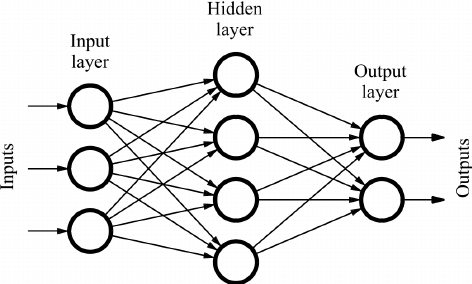
\includegraphics[width=0.5\textwidth]{figures/FFNN.png}
	\caption{High level architecture of a feedforward neural network ~\parencite{nnimagesource}}
	\label{fig:ffnn}
\end{figure}


'The goal of a feedforward network is to approximate some function $f^{*}$ .For example, for a classifier,  $y=f^{*}(\boldsymbol{x})$ maps an input  $\boldsymbol{x}$ to a category y .  A feedforward network  defines a mapping $\boldsymbol{y}=f(\boldsymbol{x} ; \boldsymbol{\theta})$ and learns the value of the parameters $\boldsymbol{\theta}$  that result in the best function approximation" \cite{Goodfellow-et-al-2016}. For a linear model, $\theta$ would consist of $\boldsymbol{w}$ and $\boldsymbol{b}$. The equation for one layer would be

\begin{equation}
f(\boldsymbol{x} ; \boldsymbol{w}, b)=\sigma(\boldsymbol{x}^{\top} \boldsymbol{w}+b) .
\label{eq:nn-one-layer}
\end{equation} 

In the equation \eqref{eq:nn-one-layer}, $\sigma$ refers to the activation function, $\boldsymbol{w}$ represents the weighting matrix that is learned and $\boldsymbol{b}$ is some bias. These layers can be connected to form the deep neural network, where $\boldsymbol{x}$ denotes the output of the previous layer. Finally, a loss function, that measures the deviation between the predicted label and the true label is minimized by the network.

Neural networks are already used to recommend videos on YouTube \cite{covington2016deep}, recommend movies \cite{christakou2007hybrid} and recommend Android applications on Google Play store \cite{cheng2016wide}. The advantage of neural networks compared to other supervised learning methods is the fact that they can learn and generalize from labeled data without much of adjustments \cite{maind2014research}.


\subsection{Embeddings}\label{research:embeddings}

Embeddings can be used to reduce dimensionality with neural networks. Embeddings layer of a network only accepts the indices of the desired skills and outputs a much smaller dimension. This technique is also used in this thesis \cite{gal2016theoretically}.





\section{Summary}


In the scope of this chapter, we gave detailed information about the types of recommender systems with a focus on the content-based recommendation. Then, we listed the evaluation properties that can lead to user satisfaction. Next, we disclosed the property that we chose, which is the diversity and illustrated how diversity could be calculated. Lastly, a short introduction to the neural networks is given.
